\documentclass[10pt]{article}
\usepackage[letterpaper,top=0.54in,bottom=0.54in,left=0.66in,right=0.66in]{geometry}
\usepackage[T1]{fontenc}
\usepackage[utf8]{inputenc}
\usepackage[hidelinks]{hyperref}
\usepackage{microtype}
\usepackage{xcolor}
\usepackage{tikz}
\usetikzlibrary{arrows.meta,calc,positioning,shapes.geometric,backgrounds,fit}
\usepackage{adjustbox}

\definecolor{ink}{HTML}{263640}
\definecolor{midgray}{HTML}{6C7780}
\definecolor{softgray}{HTML}{F3F5F6}
\definecolor{blueLine}{HTML}{6287AD}
\definecolor{blueFill}{HTML}{DFEAF4}
\definecolor{greenLine}{HTML}{6C967D}
\definecolor{greenFill}{HTML}{E2EEE5}
\definecolor{violetLine}{HTML}{8B79A5}
\definecolor{violetFill}{HTML}{EBE4F2}
\definecolor{goldLine}{HTML}{B18A38}
\definecolor{goldFill}{HTML}{F7EED8}
\definecolor{coralLine}{HTML}{C97E70}
\definecolor{coralFill}{HTML}{F5E5E1}

\pagestyle{empty}
\setlength{\parindent}{0pt}
\setlength{\parskip}{0.28em}
\setlength{\emergencystretch}{1.5em}
\linespread{1.01}

\newcommand{\interesthead}[2]{%
  \vspace{0.12em}\noindent{\large\bfseries\color{#1}#2}\par\vspace{0.05em}%
}

\begin{document}

\begin{center}
{\Large\bfseries Research Interests}\par
\vspace{0.02em}
{\normalsize Tran Duc Le}
\end{center}

\vspace{0.05em}

I study how networked systems can be defended when evidence is incomplete, operational resources are limited, and some defensive decisions are increasingly automated. This perspective grew from my doctoral work on wireless networking, where contention, interference, and protocol behavior led naturally to questions of resilience and adversarial behavior. My research now centers on two established themes, \textbf{network and systems security} and \textbf{deployable security analytics}, with an emerging extension into \textbf{AI-enabled cyber defense}. The common thread is practical: understand system behavior, derive defensible evidence, turn that evidence into usable controls, and automate only where doing so remains transparent and governable.



\interesthead{ink}{Network and Systems Security}

\par\vspace{0.5em}
\noindent\begin{adjustbox}{max width=0.85\linewidth, center}
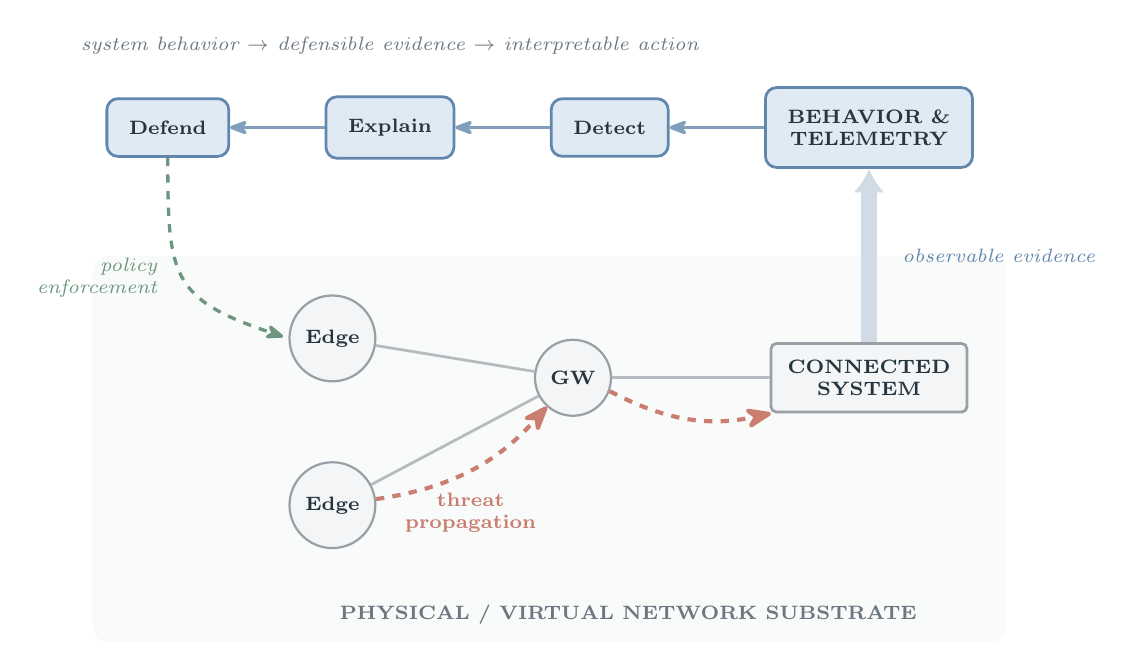
\begin{tikzpicture}[node distance=1.2cm and 1.2cm, >=Latex]
  \tikzset{
    base-node/.style={font=\scriptsize\bfseries, text=ink, align=center},
    net-node/.style={base-node, circle, fill=softgray, draw=midgray!70, line width=0.8pt, inner sep=4pt},
    net-srv/.style={base-node, rectangle, rounded corners=2pt, fill=softgray, draw=midgray!70, line width=1pt, inner sep=6pt},
    pipe-node/.style={base-node, rectangle, rounded corners=4pt, fill=blueFill, draw=blueLine, line width=1pt, inner sep=8pt},
    threat-arrow/.style={-{Stealth[scale=1.2, round]}, line width=1.5pt, coralLine},
    flow-arrow/.style={-{Stealth[scale=1.0, round]}, line width=1.2pt, blueLine!80},
    feedback-arrow/.style={-{Stealth[scale=1.0, round]}, line width=1.2pt, greenLine, dashed, shorten >=2pt},
    extract-beam/.style={-{Latex[length=3mm,width=4mm]}, line width=6pt, draw=blueLine!30}
  }

  % SUBSTRATE: Network Environment
  \begin{scope}[local bounding box=netenv]
    \node[net-node] (c1) {Edge};
    \node[net-node, below=1.0cm of c1] (c2) {Edge};
    \node[net-node, right=2.0cm of c1, yshift=-0.5cm] (gw) {GW};
    \node[net-srv, right=2.0cm of gw] (srv) {CONNECTED\\SYSTEM};

    \draw[midgray!50, line width=1pt] (c1) -- (gw);
    \draw[midgray!50, line width=1pt] (c2) -- (gw);
    \draw[midgray!50, line width=1pt] (gw) -- (srv);
    
    % Threat Propagation routed along the nodes
    \draw[threat-arrow, dashed, bend right=20] (c2) to node[below, font=\scriptsize\bfseries, text=coralLine, align=center, yshift=-0.15cm] {threat\\propagation} (gw);
    \draw[threat-arrow, dashed, bend right=20] (gw) to (srv);
  \end{scope}
  
  \begin{scope}[on background layer]
    \fill[softgray!50, rounded corners=6pt] ($(netenv.south west)+(-2.5,-1.2)$) rectangle ($(netenv.north east)+(0.5,0.5)$);
  \end{scope}

  \node[font=\scriptsize\bfseries, text=midgray, below=0.6cm of netenv] {PHYSICAL / VIRTUAL NETWORK SUBSTRATE};

  % EXTRACTION BEAM
  \node[pipe-node, above=2.2cm of srv] (evidence) {BEHAVIOR \&\\TELEMETRY};
  
  \draw[extract-beam] (srv.north) -- (evidence.south);
  \node[font=\scriptsize\itshape, text=blueLine, right=0.3cm of srv.north, yshift=1.1cm] {observable evidence};

  % PIPELINE: Defense Analytics (Flows Right to Left to close the loop)
  \node[pipe-node, left=1.2cm of evidence] (detect) {Detect};
  \node[pipe-node, left=1.2cm of detect] (explain) {Explain};
  \node[pipe-node, left=1.2cm of explain] (defend) {Defend};

  \draw[flow-arrow] (evidence) -- (detect);
  \draw[flow-arrow] (detect) -- (explain);
  \draw[flow-arrow] (explain) -- (defend);
  
  % Feedback to edge
  \draw[feedback-arrow] (defend.south) .. controls +(0,-1.5) and +(-1.5, 0.5) .. (c1.west) node[midway, left, font=\scriptsize\itshape, text=greenLine, align=right, xshift=-0.2cm] {policy\\enforcement};

  \node[font=\scriptsize\itshape, text=midgray, above=0.4cm of explain] {system behavior $\rightarrow$ defensible evidence $\rightarrow$ interpretable action};
\end{tikzpicture}
\end{adjustbox}
\par\vspace{0.5em}

\vspace{-0.18em}
My core research examines how attacks emerge from network and system behavior and how defensive evidence can remain faithful to that behavior. Early work modeled malware propagation in vehicular and Wi-Fi networks; more recent studies address IoT/IIoT intrusion detection, malware traffic analysis, and explainable intrusion triage. Across this work, I have remained interested in protocol-aware and behavior-aware defense: how to detect attacks while preserving evidence that helps explain what happened and supports a practical response.

\interesthead{ink}{Deployable Security Analytics}

\par\vspace{0.5em}
\noindent\begin{adjustbox}{max width=0.85\linewidth, center}
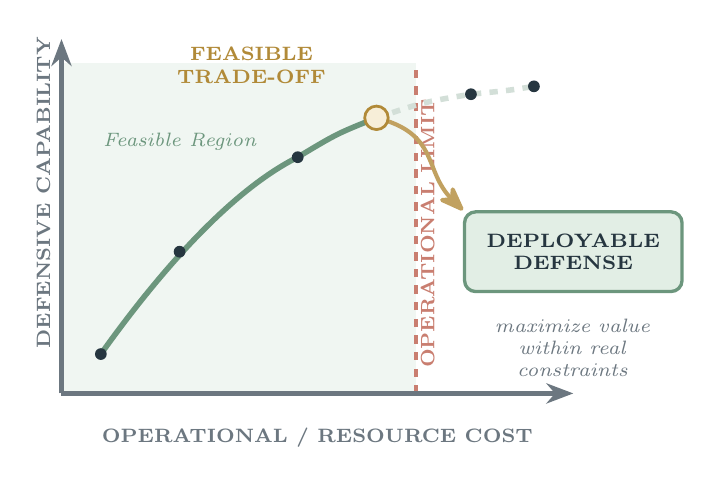
\begin{tikzpicture}[>=Latex]
  \tikzset{
    base-node/.style={font=\scriptsize\bfseries, text=ink, align=center},
    axis-line/.style={-{Stealth[scale=1.0]}, line width=1.5pt, midgray},
    limit-line/.style={coralLine, line width=1.5pt, dashed},
    frontier-line/.style={greenLine, line width=2pt},
    infeasible-line/.style={greenLine!30, line width=2pt, dashed},
    point-node/.style={circle, fill=ink, inner sep=1.5pt},
    optimal-node/.style={circle, fill=goldFill, draw=goldLine, inner sep=3pt, line width=1pt},
    deploy-node/.style={base-node, rectangle, rounded corners=4pt, fill=greenFill, draw=greenLine, line width=1.2pt, inner sep=8pt, text width=2.2cm}
  }

  % Axes
  \coordinate (O) at (0,0);
  \coordinate (X) at (6.5,0);
  \coordinate (Y) at (0,4.5);
  
  \draw[axis-line] (O) -- (X) node[pos=0.5, below=0.3cm, font=\scriptsize\bfseries] {OPERATIONAL / RESOURCE COST};
  \draw[axis-line] (O) -- (Y) node[pos=0.5, above=0.3cm, font=\scriptsize\bfseries, rotate=90] {DEFENSIVE CAPABILITY};

  % Feasible Region Shading
  \begin{scope}[on background layer]
    \fill[greenFill!50] (0,0) rectangle (4.5,4.2);
  \end{scope}
  \node[font=\scriptsize\itshape, text=greenLine] at (1.5, 3.2) {Feasible Region};

  % Resource Limit
  \begin{scope}[on background layer]
    \draw[limit-line] (4.5,0) -- (4.5,4.2);
  \end{scope}
  \node[font=\scriptsize\bfseries, text=coralLine, rotate=90, anchor=west] at (4.65, 0.2) {OPERATIONAL LIMIT};

  % Pareto Frontier
  \coordinate (p1) at (0.5, 0.5);
  \coordinate (p2) at (1.5, 1.8);
  \coordinate (p3) at (3.0, 3.0);
  \coordinate (p4) at (4.0, 3.5); % Optimal point on frontier near limit
  \coordinate (p5) at (5.2, 3.8); % Infeasible
  \coordinate (p6) at (6.0, 3.9); % Infeasible

  \draw[frontier-line] (p1) .. controls (1.0, 1.2) and (2.0, 2.5) .. (p3) .. controls (3.5, 3.3) .. (p4);
  \draw[infeasible-line] (p4) .. controls (4.6, 3.7) .. (p5) .. controls (5.7, 3.85) .. (p6);
  
  \node[point-node] at (p1) {};
  \node[point-node] at (p2) {};
  \node[point-node] at (p3) {};
  \node[point-node] at (p5) {};
  \node[point-node] at (p6) {};

  % Handoff to Deployable Defense
  \node[deploy-node] (deploy) at (6.5, 1.8) {DEPLOYABLE\\DEFENSE};
  
  % Draw arrow BEFORE the star so it doesn't overlap the star boundary
  \draw[-{Stealth[scale=1.2, round]}, goldLine!80, line width=1.5pt] (p4) .. controls +(0.8,-0.2) and +(-0.5,0.5) .. (deploy.north west);

  % Optimal Point (drawn after arrow)
  \node[optimal-node] (opt) at (p4) {};
  \node[font=\scriptsize\bfseries, text=goldLine, align=center, above left=0.2cm and 0.4cm of opt] {FEASIBLE\\TRADE-OFF};

  \node[font=\scriptsize\itshape, text=midgray, below=0.2cm of deploy, align=center, text width=2.5cm] {maximize value\\within real\\constraints};
\end{tikzpicture}
\end{adjustbox}
\par\vspace{0.5em}

\vspace{-0.18em}
A second line of work asks whether technically strong defenses remain useful under operational constraints. During my postdoctoral research on cybersecurity for small and medium-sized enterprises (SMEs), I examined user behavior, malicious-content threats, enterprise security analytics, and capability prioritization in organizations with limited staff, telemetry, and budgets. This work shifted my emphasis from model performance alone toward deployment feasibility: what can an organization understand, maintain, and justify? I am especially interested in methods that account for resource limits, analyst workload, explainability, and implementation cost.


\newpage
\interesthead{ink}{AI-Enabled Cyber Defense}

\par\vspace{0.5em}
\noindent\begin{adjustbox}{max width=0.85\linewidth, center}
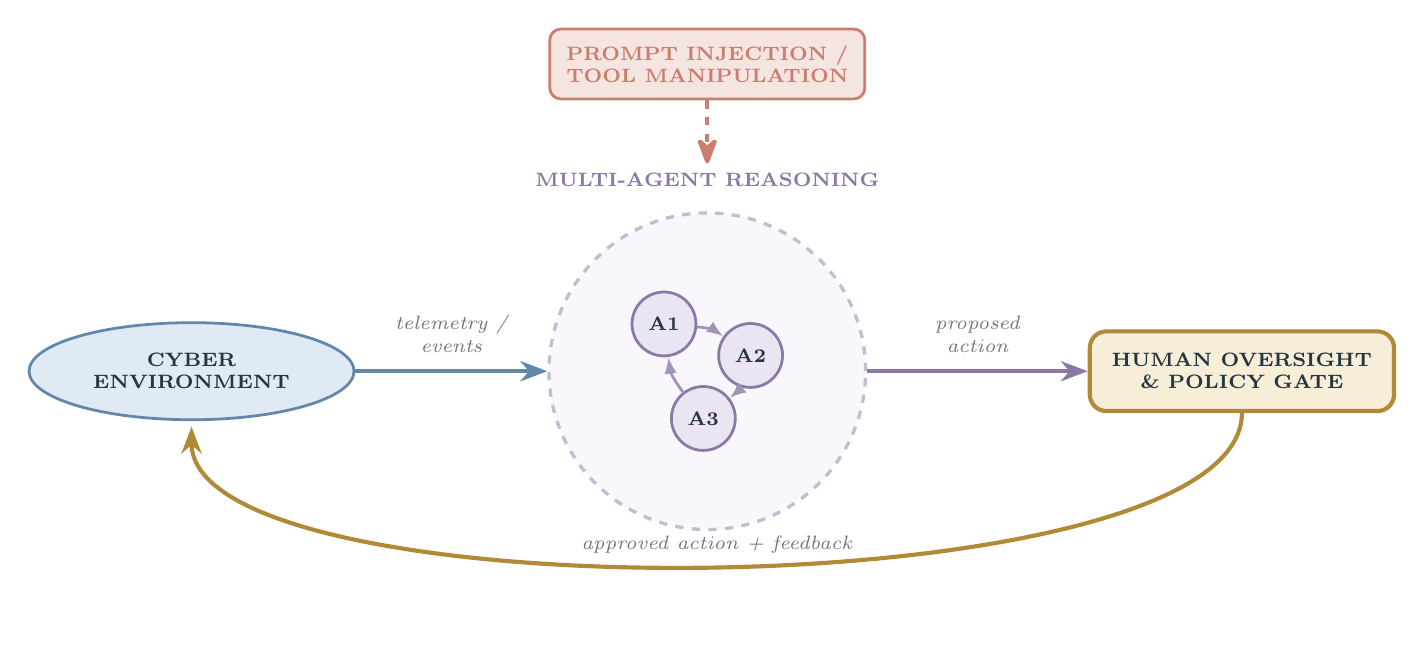
\begin{tikzpicture}[node distance=1.5cm and 2.0cm, >=Latex]
  \tikzset{
    base-node/.style={font=\scriptsize\bfseries, text=ink, align=center},
    env-node/.style={base-node, ellipse, fill=blueFill, draw=blueLine, line width=1pt, inner sep=6pt},
    agent-node/.style={circle, fill=violetFill, draw=violetLine, line width=1pt, inner sep=4pt, font=\scriptsize\bfseries, text=ink},
    gate-node/.style={base-node, rectangle, rounded corners=6pt, fill=goldFill, draw=goldLine, line width=1.5pt, inner sep=8pt},
    attack-node/.style={base-node, rectangle, rounded corners=4pt, fill=coralFill, draw=coralLine, line width=1pt, inner sep=6pt, text=coralLine},
    flow-arrow/.style={-{Stealth[scale=1.0]}, line width=1.5pt},
    attack-arrow/.style={-{Stealth[scale=1.2, round]}, coralLine, line width=1.5pt, dashed}
  }

  % Left: Environment
  \coordinate (origin) at (0,0);
  \node[env-node] (env) at (origin) {CYBER\\ENVIRONMENT};

  % Center: Multi-Agent Reasoning
  \coordinate (center-agent) at (6.5, 0);
  \node[agent-node] (a1) at ($(center-agent)+(-0.5, 0.6)$) {A1};
  \node[agent-node] (a2) at ($(center-agent)+(0.6, 0.2)$) {A2};
  \node[agent-node] (a3) at ($(center-agent)+(0.0, -0.6)$) {A3};
  
  \draw[-{Latex[scale=0.8]}, violetLine!80, line width=1pt] (a1) to[bend left=15] (a2);
  \draw[-{Latex[scale=0.8]}, violetLine!80, line width=1pt] (a2) to[bend left=15] (a3);
  \draw[-{Latex[scale=0.8]}, violetLine!80, line width=1pt] (a3) to[bend left=15] (a1);
  
  \begin{scope}[on background layer]
    \node[circle, fill=violetFill!30, draw=violetLine!50, line width=1.2pt, dashed, fit=(a1)(a2)(a3), inner sep=12pt] (agent-box) {};
  \end{scope}
  \node[font=\scriptsize\bfseries, text=violetLine] (agent-label) at ([yshift=0.4cm]agent-box.north) {MULTI-AGENT REASONING};

  % Right: Oversight
  \node[gate-node, right=2.8cm of agent-box] (gate) {HUMAN OVERSIGHT\\\& POLICY GATE};

  % Flows
  \draw[flow-arrow, blueLine] (env.east) -- (agent-box.west) node[midway, above, font=\scriptsize\itshape, text=midgray, align=center, yshift=0.1cm] {telemetry /\\events};
  \draw[flow-arrow, violetLine] (agent-box.east) -- (gate.west) node[midway, above, font=\scriptsize\itshape, text=midgray, align=center, yshift=0.1cm] {proposed\\action};
  
  % Feedback loop
  \draw[flow-arrow, goldLine, shorten >=2pt] (gate.south) .. controls +(0,-2.5) and +(0,-2.5) .. (env.south) node[midway, above, font=\scriptsize\itshape, text=midgray] {approved action + feedback};

  % Threat vector
  \node[attack-node, above=0.8cm of agent-label] (attack) {PROMPT INJECTION /\\TOOL MANIPULATION};
  \draw[attack-arrow] (attack.south) -- (agent-label.north);
\end{tikzpicture}
\end{adjustbox}
\par\vspace{0.5em}

\vspace{0.12em}
More recently, I have begun extending this systems-and-deployment perspective to AI-assisted and agentic cyber defense. My work in this area includes prompt-injection contagion in multi-agent systems and ongoing studies of tool-using agents. I am interested in the security risks that arise when AI systems interact with other agents, external tools, and operational environments, as well as in mechanisms that keep automated actions constrained and subject to human review.

\vspace{0.12em}
These interests are connected by a common concern with how security mechanisms behave in real systems and how they can support practical defense. I use network and system measurement, security modeling, machine learning, and controlled experimentation as tools rather than ends in themselves. My goal is to develop cyber-defense methods that are technically grounded, practical to deploy, and understandable to the people responsible for operating them.

\end{document}
